%        File: graph_partition.tex
%     Created: Sun Mar 05 08:00 PM 2017 C
% Last Change: Sun Mar 05 08:00 PM 2017 C
%

\documentclass{beamer}
%\usetheme{Boadilla}
\usetheme{Madrid}

\title{Multilevel $k$-way Partitioning Scheme for Irregular Graphs}
\subtitle{G. Karypis and V. Kumar}
\institute{University of Minnesota}
\date{March 7, 2017}
\author{Trevor Steil}

\mode<presentation>{}

\setbeamertemplate{navigation symbols}{}

%\usepackage{amsmath}
%\usepackage{amsthm}
%\usepackage{amssymb}
%\usepackage{esint}
%\usepackage{enumitem}
\usepackage[plain]{algorithm}
\usepackage{algorithmic}
%\usepackage{algorithmicx}
%\usepackage{algpseudocode}
%\usepackage{bbm}
%\usepackage{xcolor}
\usepackage{graphicx}
\usepackage{tikz}
\usepackage{caption}

%\newtheorem{theorem}{Theorem}[section]
%\newtheorem{corollary}{Corollary}[section]
%\newtheorem{proposition}{Proposition}[section]
%\newtheorem{lemma}{Lemma}[section]
%\newtheorem*{claim}{Claim}
%%\newtheorem*{problem}{Problem}
%%\newtheorem*{lemma}{Lemma}
%\newtheorem{definition}{Definition}[section]
%
%\newcommand{\R}{\mathbb{R}}
%\newcommand{\N}{\mathbb{N}}
%\newcommand{\C}{\mathbb{C}}
%\newcommand{\Z}{\mathbb{Z}}
%\newcommand{\Q}{\mathbb{Q}}
%\newcommand{\E}{\mathbb{E}}
%\newcommand{\supp}[1]{\mathop{\mathrm{supp}}\left(#1\right)}
%\newcommand{\lip}[1]{\mathop{\mathrm{Lip}}\left(#1\right)}
%\newcommand{\curl}{\mathrm{curl}}
%\newcommand{\la}{\left \langle}
%\newcommand{\ra}{\right \rangle}
%\renewcommand{\vec}[1]{\mathbf{#1}}
%\renewcommand{\div}{\mathrm{div}}
%
%\newenvironment{problem}{\textbf{Problem.}}
%
%\newenvironment{solution}[1][]{\emph{Solution #1}}
%
%\algnewcommand{\Or}{\textbf{ or }}
%\algnewcommand{\And}{\textbf{ or }}

\begin{document}

\begin{frame}
  \titlepage
\end{frame}

\begin{frame}
  \frametitle{Table of Contents}
  \tableofcontents
\end{frame}

\section{Introduction}
\begin{frame}
  \frametitle{Graph Partitioning}

  Given a graph $G = (V, E)$ with $|V|=n$, we want to partition $V$ into subsets $V_1, \dots, V_k$ such that
  \begin{itemize}
    \item $V_i \cap V_j = \emptyset$ for $i \neq j$
    \item $\bigcup_{i=1}^k V_i = V$
    \item $|V_i| = \frac{n}{k}$ for all $i$ (approximately at least)
    \item edge-cut is minimized
  \end{itemize}
  where edge-cut is the number of edges between vertices of different subsets of partition
\end{frame}

\begin{frame}
  \frametitle{Uses of Graph Partitioning}

  \begin{itemize}
    \item Assigning tasks to processors in parallel computation
    \item Sparse matrix-vector multiplication
  \end{itemize}

  \begin{figure}
    \centering
    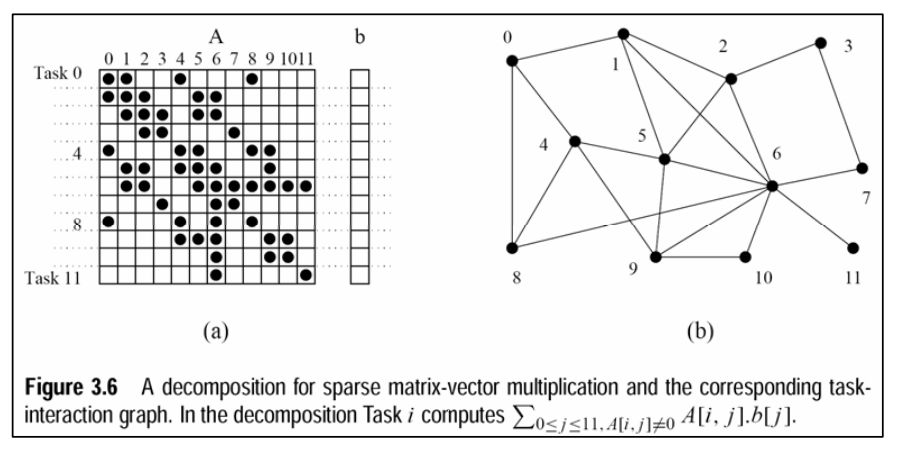
\includegraphics[width=0.7\textwidth]{./sparse.png}
    \caption*{From \textit{Introduction to Parallel Computing} by A. Grama, A. Gupta, G. Karypis, and V. Kumar}
  \end{figure}
\end{frame}

\begin{frame}
  \frametitle{Recursive Bisection}

  Can repeatedly partition graph in two
  \begin{itemize}
    \item Recursive Bisection
    \item Recursive nature leads to logarithmic term in running time ($O(|E| \log k)$)
    \item Partitioning graph in two is still difficult to do.
  \end{itemize}

\end{frame}

\begin{frame}
  \frametitle{Multilevel k-Way Partitioning}

  \begin{block}{Idea:}
    It is easier to partition smaller graphs
  \end{block}

  Instead of trying to partition original graph, try reducing to a smaller graph.

\end{frame}

\section{Algorithm}

\begin{frame}
  \frametitle{Basic Algorithm Steps}

  \begin{enumerate}
    \item
      Successively coarsen graph
    \item
      Partition coarsest graph
    \item
      Uncoarsen graph and refine partition
  \end{enumerate}

  \begin{figure}
    \centering
    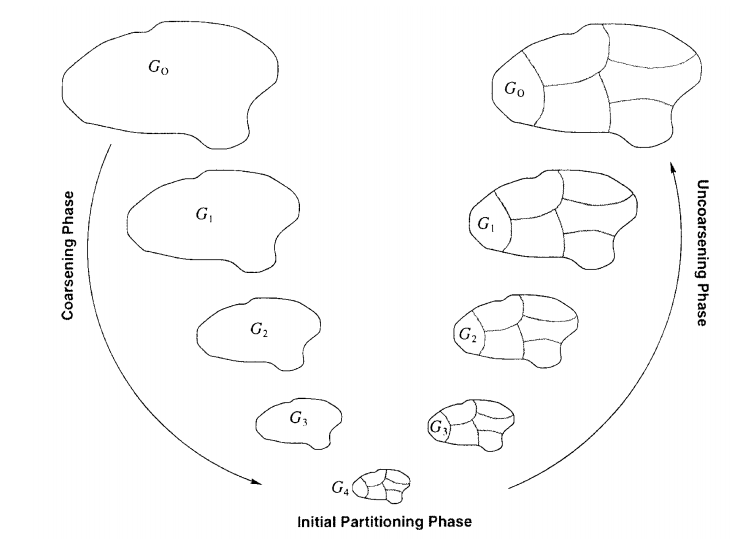
\includegraphics[width=0.7\textwidth]{./multilevel.png}
  \end{figure}

\end{frame}

\subsection{Coarsening Phase}

\begin{frame}
  \frametitle{Coarsening Phase}

  Let $G_0 = (V_0, E_0) = (V,E)$ be the original graph. Want a sequence $G_i = (V_i, E_i)$ with $|V_i| < |V_{i-1}|$.

  \vspace{.5cm}

  Need to add weights to vertices and edges to keep track of number of original vertices and edges are in each coarsened vertex and edge.

\end{frame}

\begin{frame}
  \frametitle{Use of Matchings}

  Collapse along edges of a matching to coarsen graph

  Randomized Matching Algorithm:
  \begin{itemize}
    \item Visit vertices in random order
    \item At each unmatched vertex, choose a random unmatched neighbor (if any exist)
    \item Add corresponding edge to matching
  \end{itemize}

  \begin{center}
  \begin{tikzpicture}
    [scale=1,auto=left,every node/.style={circle,fill=blue!20}]
    \node[label=1] (n1) at (1,3) {};
    \node[label=2] (n2) at (3,3) {};
    \node[label=3] (n3) at (4,2) {};
    \node[label=below:4] (n4) at (3,1) {};
    \node[label=below:5] (n5) at (1,1) {};

    \draw (n1) -- (n2);
    \draw (n1) -- (n5);
    \draw (n2) -- (n3);
    \draw (n2) -- (n4);
    \draw (n3) -- (n4);
    \draw (n4) -- (n5);

    \node[fill=white] (n1') at (9,3) {};
    \node[fill=white] (n2') at (10,1) {};
    \node[fill=white] (n3') at (8,1) {};
  \end{tikzpicture}
  \end{center}

  Visit Order: 1, 2, 3, 4, 5

\end{frame}

\begin{frame}[noframenumbering]
  \frametitle{Use of Matchings}

  Collapse along edges of a matching to coarsen graph

  Randomized Matching Algorithm:
  \begin{itemize}
    \item Visit vertices in random order
    \item At each unmatched vertex, choose a random unmatched neighbor (if any exist)
    \item Add corresponding edge to matching
  \end{itemize}

  \begin{center}
  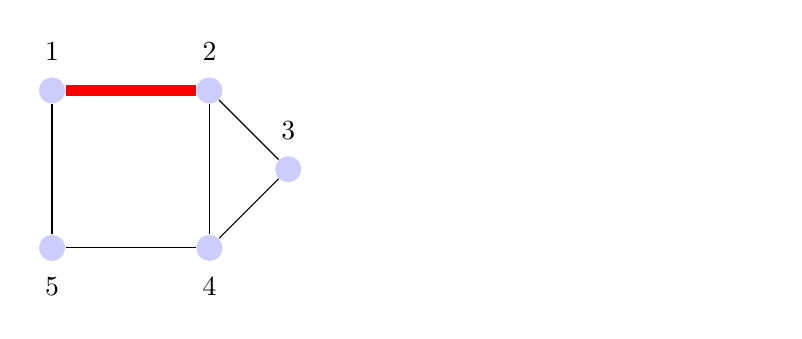
\begin{tikzpicture}
    [scale=1,auto=left,every node/.style={circle,fill=blue!20}]
    \node[label=1] (n1) at (1,3) {};
    \node[label=2] (n2) at (3,3) {};
    \node[label=3] (n3) at (4,2) {};
    \node[label=below:4] (n4) at (3,1) {};
    \node[label=below:5] (n5) at (1,1) {};

    \draw [red, line width=4pt] (n1) -- (n2);
    \draw (n1) -- (n5);
    \draw (n2) -- (n3);
    \draw (n2) -- (n4);
    \draw (n3) -- (n4);
    \draw (n4) -- (n5);

    \node[fill=white] (n1') at (9,3) {};
    \node[fill=white] (n2') at (10,1) {};
    \node[fill=white] (n3') at (8,1) {};
  \end{tikzpicture}
  \end{center}

  Visit Order: 1, 2, 3, 4, 5

\end{frame}

\begin{frame}[noframenumbering]
  \frametitle{Use of Matchings}

  Collapse along edges of a matching to coarsen graph

  Randomized Matching Algorithm:
  \begin{itemize}
    \item Visit vertices in random order
    \item At each unmatched vertex, choose a random unmatched neighbor (if any exist)
    \item Add corresponding edge to matching
  \end{itemize}

  \begin{center}
  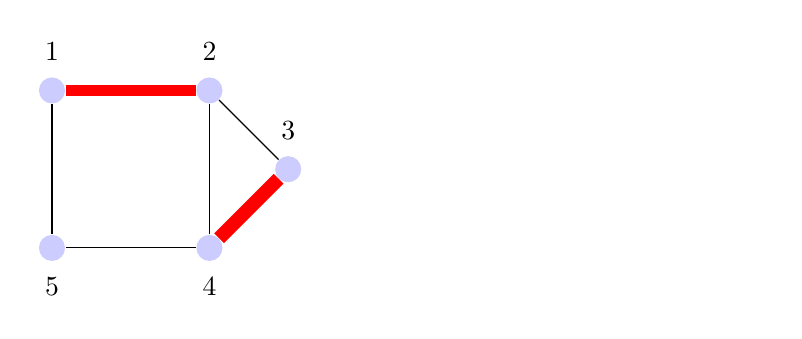
\begin{tikzpicture}
    [scale=1,auto=left,every node/.style={circle,fill=blue!20}]
    \node[label=1] (n1) at (1,3) {};
    \node[label=2] (n2) at (3,3) {};
    \node[label=3] (n3) at (4,2) {};
    \node[label=below:4] (n4) at (3,1) {};
    \node[label=below:5] (n5) at (1,1) {};

    \draw [red, line width=4pt] (n1) -- (n2);
    \draw (n1) -- (n5);
    \draw (n2) -- (n3);
    \draw (n2) -- (n4);
    \draw [red, line width=5pt] (n3) -- (n4);
    \draw (n4) -- (n5);

    \node[fill=white] (n1') at (9,3) {};
    \node[fill=white] (n2') at (10,1) {};
    \node[fill=white] (n3') at (8,1) {};
  \end{tikzpicture}
  \end{center}

  Visit Order: 1, 2, 3, 4, 5

\end{frame}

\begin{frame}[noframenumbering]
  \frametitle{Use of Matchings}

  Collapse along edges of a matching to coarsen graph

  Randomized Matching Algorithm:
  \begin{itemize}
    \item Visit vertices in random order
    \item At each unmatched vertex, choose a random unmatched neighbor (if any exist)
    \item Add corresponding edge to matching
  \end{itemize}

  \begin{center}
  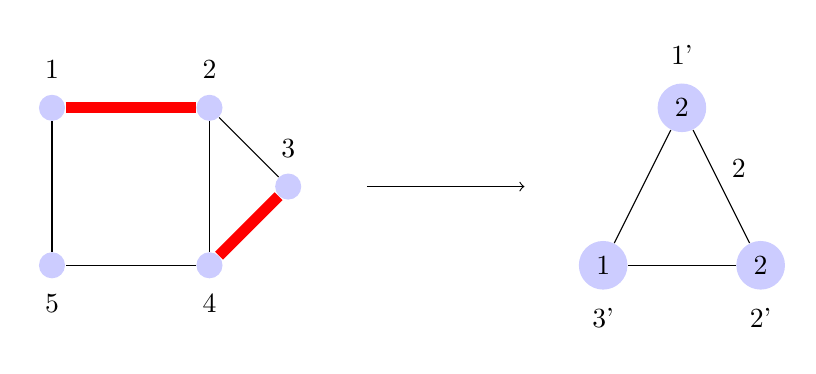
\begin{tikzpicture}
    [scale=1,auto=left,every node/.style={circle,fill=blue!20}]
    \node[label=1] (n1) at (1,3) {};
    \node[label=2] (n2) at (3,3) {};
    \node[label=3] (n3) at (4,2) {};
    \node[label=below:4] (n4) at (3,1) {};
    \node[label=below:5] (n5) at (1,1) {};

    \draw [red, line width=4pt] (n1) -- (n2);
    \draw (n1) -- (n5);
    \draw (n2) -- (n3);
    \draw (n2) -- (n4);
    \draw [red, line width=4pt] (n3) -- (n4);
    \draw (n4) -- (n5);

    \draw[->] (5,2) -- (7,2);

    \node[label=1'] (n1') at (9,3) {2};
    \node[label=below:2'] (n2') at (10,1) {2};
    \node[label=below:3'] (n3') at (8,1) {1};

    \draw (n1') -- (n2') node [midway, fill=white, opacity=0, text opacity=1] {2};
    \draw (n1') -- (n3');
    \draw (n2') -- (n3');
  \end{tikzpicture}
  \end{center}

  Visit Order: 1, 2, 3, 4, 5

\end{frame}

\begin{frame}
  \frametitle{Heavy Edge Matching}

  Coarsening step reduces total edge weight by edge weights of matching
  \begin{itemize}
    \item To minimize edge cut, choose edges that maximize weight of matching
  \end{itemize}

  Algorithm:
  \begin{itemize}
    \item Visit vertices in random order
    \item At each unmatched vertex, choose unmatched neighbor along heaviest edge
    \item Add corresponding edge to matching
  \end{itemize}

  Has same computational complexity as randomized matching ($O(|E|)$)
\end{frame}

\subsection{Initial Partitioning}

\begin{frame}
  \frametitle{Initial Partitioning}

  Partition $G_n=(V_n,E_n)$ into $k$ subsets after several coarsening steps using any method
  \begin{itemize}
    \item i.e. recursive bisection, spectral bisection, etc.
  \end{itemize}

  \vspace{1cm}

  Want vertex weights to be approximately equal among partitions

\end{frame}

\subsection{Uncoarsening Phase}

\begin{frame}
  \frametitle{Uncoarsening Phase}

  Basic Steps:
  \begin{itemize}
    \item Take partitioning of $G_i$ to a partitioning of $G_{i-1}$ by reversing the matching and collapse of coarsening that sent $G_{i-1}$ to $G_i$.
    \item Refine partition to have lower edge cut
  \end{itemize}

  Several refining algorithms exist, based on various heuristics.

\end{frame}

\begin{frame}
  \frametitle{Kernighan-Lin (KL) Algorithm}

  Used for bisection (not $k$-way partitioning)

  For a vertex $v$, let $gain(v)$ be the decrease in edge-cut when $v$ is moved to other partition.

  \begin{block}{KL Algorithm}
    \begin{algorithm}[H]
      \begin{algorithmic}[1]
        \STATE Compute $gain$ for all vertices
        \STATE Create priority queue for each partition based on $gain$
        \FOR {$v$ with highest gain}
        \STATE Move $v$ to other partition
        \STATE Update $gain$ of neighbors of $v$
        \STATE Record current edge-cut
        \STATE Lock $v$ so it cannot be moved again
        \ENDFOR
        \STATE Choose configuration that had lowest edge-cut
      \end{algorithmic}
    \end{algorithm}
  \end{block}

\end{frame}

\begin{frame}
  \frametitle{Maintaining Balanced Partitions}

  Let $W_i[j] = $ weight of partition $j$ in $G_i$, $W^{min} = 0.9|V_0|/k$ and $W^{max} = C |V_0|/k$ for some $C$. Only allow vertex $v$ to move from partition $a$
  to partition $b$ if
  \[ W_i[b] + w(v) \leq W^{max} \]
  and
  \[ W_i[a] - w(v) \geq W^{min} \]
  where $w(v)$ is the weight of vertex $v$.
\end{frame}

\begin{frame}
  \frametitle{KL for $k$-Way Partitioning}

  Using the straightforward generalization is not practical for large $k$
  \begin{itemize}
    \item Each vertex is in one of $k$ subsets and can move to any of $k-1$ other subsets
    \item Requires $k(k-1)$ queues
  \end{itemize}

\end{frame}

\begin{frame}
  \frametitle{Lookahead in KL for Bisections}

  By maintaining queues and moving all vertices, groups of vertices can cross boundary when some individual moves will lead to negative gain

  \begin{figure}
    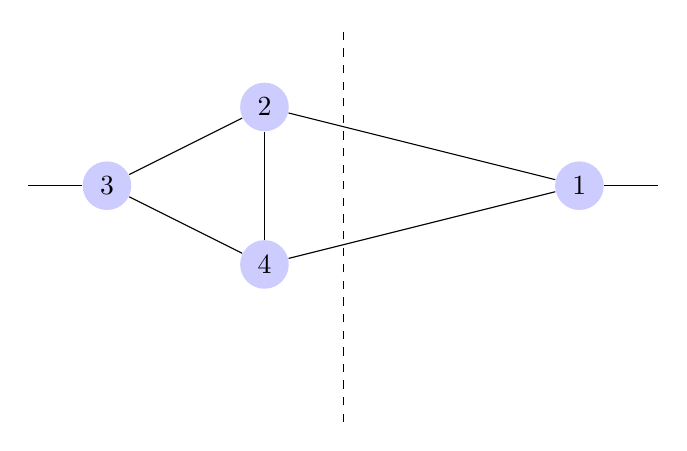
\begin{tikzpicture}
      [every node/.style={circle,fill=blue!20}]
      \node (n1) at (7,3) {1};
      \node (n2) at (3,4) {2};
      \node (n3) at (1,3) {3};
      \node (n4) at (3,2) {4};

      \foreach \from/\to in {n1/n2, n1/n4, n2/n3, n2/n4, n3/n4}
      \draw (\from) -- (\to);

      \draw [dashed]  (4,0) -- (4,5);
      \draw (n1) -- (8,3);
      \draw (n3) -- (0,3);
    \end{tikzpicture}
    \caption*{Edge-Cut:2}
  \end{figure}

\end{frame}

\begin{frame}[noframenumbering]
  \frametitle{Lookahead in KL for Bisections}

  By maintaining queues and moving all vertices, groups of vertices can cross boundary when some individual moves will lead to negative gain

  \begin{figure}[noframenumbering]
    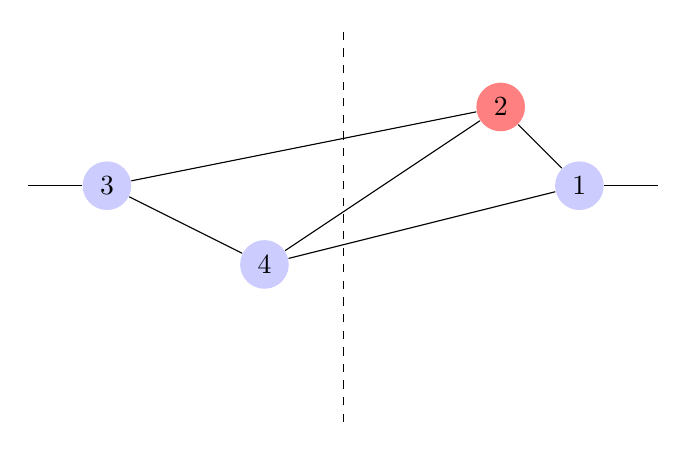
\begin{tikzpicture}
      [every node/.style={circle,fill=blue!20}]
      \node (n1) at (7,3) {1};
      \node [fill=red!50] (n2) at (6,4) {2};
      \node (n3) at (1,3) {3};
      \node (n4) at (3,2) {4};

      \foreach \from/\to in {n1/n2, n1/n4, n2/n3, n2/n4, n3/n4}
      \draw (\from) -- (\to);

      \draw [dashed]  (4,0) -- (4,5);
      \draw (n1) -- (8,3);
      \draw (n3) -- (0,3);
    \end{tikzpicture}
    \caption*{Edge-Cut:3}
  \end{figure}

\end{frame}

\begin{frame}[noframenumbering]
  \frametitle{Lookahead in KL for Bisections}

  By maintaining queues and moving all vertices, groups of vertices can cross boundary when some individual moves will lead to negative gain

  \begin{figure}
    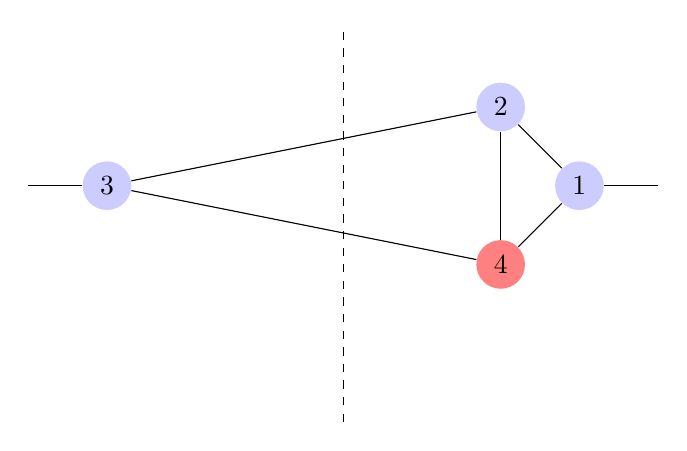
\begin{tikzpicture}
      [every node/.style={circle,fill=blue!20}]
      \node (n1) at (7,3) {1};
      \node (n2) at (6,4) {2};
      \node (n3) at (1,3) {3};
      \node [fill=red!50] (n4) at (6,2) {4};

      \foreach \from/\to in {n1/n2, n1/n4, n2/n3, n2/n4, n3/n4}
      \draw (\from) -- (\to);

      \draw [dashed]  (4,0) -- (4,5);
      \draw (n1) -- (8,3);
      \draw (n3) -- (0,3);
    \end{tikzpicture}
    \caption*{Edge-Cut:2}
  \end{figure}

\end{frame}

\begin{frame}[noframenumbering]
  \frametitle{Lookahead in KL for Bisections}

  By maintaining queues and moving all vertices, groups of vertices can cross boundary when some individual moves will lead to negative gain

  \begin{figure}
    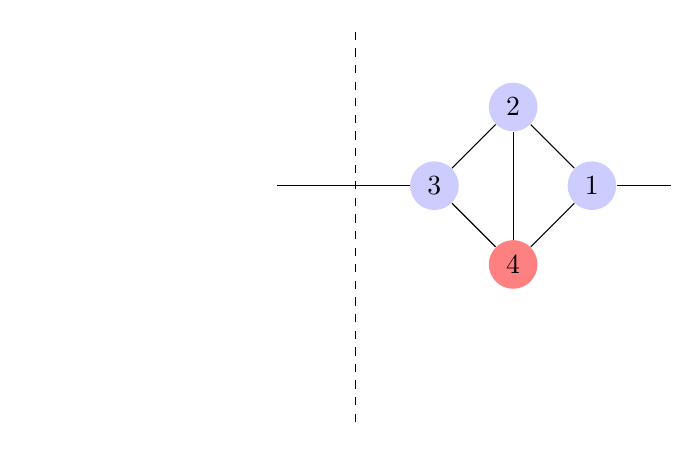
\begin{tikzpicture}
      [every node/.style={circle,fill=blue!20}]
      \node (n1) at (7,3) {1};
      \node (n2) at (6,4) {2};
      \node (n3) at (5,3) {3};
      \node [fill=red!50] (n4) at (6,2) {4};
      \node [fill=white,opacity=0] (n5) at (0,3) {};

      \foreach \from/\to in {n1/n2, n1/n4, n2/n3, n2/n4, n3/n4}
      \draw (\from) -- (\to);

      \draw [dashed]  (4,0) -- (4,5);
      \draw (n1) -- (8,3);
      \draw (n3) -- (3,3);
    \end{tikzpicture}
    \caption*{Edge-Cut:1}
  \end{figure}

\end{frame}

\begin{frame}
  \frametitle{Lookahead for $k$-way Partitioning}

  Heuristically, moving groups of vertices can be accomplished by moving a single vertex in a coarser graph

  A coarser partitioning of the previous example:

  \begin{figure}
    \begin{tikzpicture}
      [every node/.style={circle,fill=blue!20}]
      \node [label=1] (n1) at (5,3) {1};
      \node [label=2'] (n2) at (2,3) {3};
      \node [fill=white] (invis) at (0,3) {};

      \draw [dashed] (3,0) -- (3,5);
      \draw (n1) -- (n2) node [midway, label={[yshift=-.2cm]2}, fill=white, opacity=0, text opacity=1] {};
      \draw (n1) -- (6,3);
      \draw (n2) -- (1,3);
    \end{tikzpicture}
    \caption*{Edge-Cut: 2}
  \end{figure}

\end{frame}

\begin{frame}[noframenumbering]
  \frametitle{Lookahead for $k$-way Partitioning}

  Heuristically, moving groups of vertices can be accomplished by moving a single vertex in a coarser graph

  A coarser partitioning of the previous example:

  \begin{figure}
    \begin{tikzpicture}
      [every node/.style={circle,fill=blue!20}]
      \node [label=1] (n1) at (5,3) {1};
      \node [label=2'] (n2) at (4,3) {3};
      \node [fill=white] (invis) at (0,3) {};

      \draw [dashed] (3,0) -- (3,5);
      \draw (n1) -- (n2) node [midway, label={[yshift=-.2cm]2}, fill=white, opacity=0, text opacity=1] {};
      \draw (n1) -- (6,3);
      \draw (n2) -- (2,3);
    \end{tikzpicture}
    \caption*{Edge-Cut: 1}
  \end{figure}

\end{frame}

\begin{frame}[fragile]
  \frametitle{Greedy Refinement}

  \begin{block}{Greedy Refinement pseudocode}
  \begin{algorithm}[H]
    \begin{algorithmic}[1]
      \FOR{ vertices $v$ on boundary of partitions}
      \STATE{ Move $v$ to the subset that minimizes edge-cut while maintaining balance condition }
      \ENDFOR
    \end{algorithmic}
  \end{algorithm}
\end{block}

This refinement step is performed iteratively.

\end{frame}

\begin{frame}
  \frametitle{Completed Algorithm}

  \begin{block}{Multilevel $k$-way Partitioning (MLkP) Algorithm}
    \begin{enumerate}
      \item Coarsen graph using Heavy Edge Matching
      \item Partition coarse graph
      \item Uncoarsen graph and refine partition using Greedy Refinement
    \end{enumerate}
  \end{block}

\end{frame}

\section{Results}

\begin{frame}
  \frametitle{Performance}

  MLkP:
  \begin{itemize}
    \item produces partitions of the same quality as Multilevel Recursive Bisection (MLRB)
    \item runs approximately 3x faster than MLRB
  \end{itemize}

\end{frame}

\begin{frame}
  \frametitle{References}

  \begin{itemize}
    \item G. Karypis, V. Kumar. ``Multilevel $k$-way Partitioning Scheme for Irregular Graphs.'' Journal of Parallel and Distributed Computing, 1998.

    \item A. Grama, A. Gupta, G. Karypis, V. Kumar. ``Introduction to Parallel Computing.'' Addison-Wesley, 2003.

    \item B. Hendrickson, R. Leland. ``A Multilevel Algorithm for Partitioning Graphs.'' Supercomputing '95 Proceedings of the 1995 ACM/IEEE
      Conference on Supercomputing, 1995.
  \end{itemize}
\end{frame}

\end{document}


